\documentclass[11pt,a4paper]{report}

% Aberstwyth dissertation LaTeX Template
% Authors: Dr. Hannah Dee (hmd1@aber.ac.uk), Neil Taylor (nst@aber.ac.uk)
% This has been adapted from the Leeds Thesis template and the 
% Group Project template for Computer Science in Aberystywth University.
% 
% All comments and suggestions welcome.
%
% Template designed to be used with pdflatex: it may need alteration to
% run with a different LaTeX engine.
%
% Note - this is offered as a starting point for your work. You are not 
% required to use this template and can choose to create your own document 
% without it. 

% To build document on the unix command line, run four commands:
 
% pdflatex dissertation
% bibtex dissertation
% pdflatex dissertation
% pdflatex dissertation

% you will end up with dissertation.pdf 
\usepackage{mmp}

% the following packages are used for citations - You only need to include one. 
%
% Use the cite package if you are using the numeric style (e.g. IEEEannot). 
% Use the natbib package if you are using the author-date style (e.g. authordate2annot). 
% Only use one of these and comment out the other one. 
\usepackage{cite}
%\usepackage{natbib}

\usepackage{textcomp}
\usepackage{graphicx}
\usepackage{tabu}
\usepackage{pdfpages}

% Use the following to selectively exclude chapters
%\includeonly{cover,abstract,acknowledge,declare,chapter1,chapter2}

\begin{document}

% all of the include directives below refer to tex files
% so 
\title{Using the Pepper’s Ghost Pyramid technique to create real-time holograms for a charades style game}

% Your name
\author{Elliot Oram}

% Your email 
\authoremail{elo9@aber.ac.uk}

\degreeschemecode{G401} %e.g. G400 
\degreeschemetitle{Computer Science} % e.g. Computer Science
\degreetype{BSc}

\modulecode{CS39440} % i.e. CS39440, CC39440, CS39620
\moduletitle{Major Project} % i.e. Major Project or Minor Project

\date{28th February 2017} % i.e. the date of this version of the report

\status{Draft} % Use draft until you create the release version. Then, change this to Release.
\version{1.0}

%The title and name of your supervisor.
\supervisor{Dr. Helen Miles} 

%The email for your supervisor. 
\supervisoremail{hem23@aber.ac.uk}

\maketitle



 includes cover.tex - to change the content,
% edit the tex file

\pagenumbering{roman}

% This is the front page

\title{Using the Pepper’s Ghost Pyramid technique to create real-time holograms for a charades style game}

% Your name
\author{Elliot Oram}

% Your email 
\authoremail{elo9@aber.ac.uk}

\degreeschemecode{G401} %e.g. G400 
\degreeschemetitle{Computer Science} % e.g. Computer Science
\degreetype{BSc}

\modulecode{CS39440} % i.e. CS39440, CC39440, CS39620
\moduletitle{Major Project} % i.e. Major Project or Minor Project

\date{28th February 2017} % i.e. the date of this version of the report

\status{Draft} % Use draft until you create the release version. Then, change this to Release.
\version{1.0}

%The title and name of your supervisor.
\supervisor{Dr. Helen Miles} 

%The email for your supervisor. 
\supervisoremail{hem23@aber.ac.uk}

\maketitle



                        

% Set up page numbering
\pagestyle{empty}

% declarations of originality 
\thispagestyle{empty}

%%%
%%% You must sign the declaration of originality. 
%%%
%%% You are submitting this electronically. Therefore, to sign, you 
%%% type your name and date to replace the .... characters. 
%%%
\begin{center}
    {\LARGE\bf Declaration of originality}
\end{center}

I confirm that:

\begin{itemize}
\item{This submission is my own work, except where 
clearly indicated.}

\item{I understand that there are severe penalties for Unacceptable Academic Practice, which can lead to loss of marks or even the withholding of a degree.}
 
\item{I have read the regulations on Unacceptable Academic Practice from the University's Academic Quality and Records Office (AQRO) and the relevant sections of the current Student Handbook of the Department of Computer Science.}
 
\item{In submitting this work I understand and agree to abide by the University's regulations governing these issues.}
\end{itemize}

\vspace{2em}
Name ............................................................  \\

\vspace{1em}
Date ............................................................ \\

%%% 
%%% We would like to make a selection of final reports available to students that take 
%%% this module in future years. To enable us to do this, we require your consent. You 
%%% are not required that you do this, but if you do give your consent, then we will have 
%%% the option to select yours as one of a number of reports as examples for other 
%%% students. If you would like to give your consent, then please include the following 
%%% text and type your name and date to replace the .... characters. 
%%% 
%%% If you do not wish to give your consent, please remove this from your report. 
%%%
\vspace{1em}
\begin{center}
    {\LARGE\bf Consent to share this work}
\end{center}

By including my name below, I hereby agree to this dissertation being made available to other students and academic staff of the Aberystwyth Computer Science Department.  

\vspace{2em}
Name ............................................................  \\

\vspace{1em}
Date ............................................................ \\


               

\thispagestyle{empty}

\begin{center}
    {\LARGE\bf Acknowledgements}
\end{center}

I'd like to thank Dr. Helen Miles for her continued support throughout the duration of this project which included advise and guidance on the project context and implementation. In addition I would like to thank the members of the Aberystwyth University computer science department for their assistance in setting up the stall for my prototype demonstration at the 2017 Aberystwyth Science week. 
 % Acknowledgements
\thispagestyle{empty}

\begin{center}
    {\LARGE\bf Abstract}
\end{center}

This report describes the process followed to develop a system to create real-time holograms using the Pepper's Ghost pyramid technique and an accompanying charades game. The system was first proposed to be used at Aberystwyth university's Science week in 2018, but is also suitable to be used at any appropriate outreach events. The Pepper’s ghost pyramid technique is an excellent tool to use in outreach as it is both simple to understand how it works, and creates an impactful display. In order to improve the outreach experience for participants, the charades game is designed to provide a way to interact with the holographic system.

This report will present the purpose, technologies and processes surrounding this system. The development process followed an adapted single person FDD plan driven methodology which will be discussed in detail below. The report will also mirror the methodology and present development tasks and their completion relative to software iterations which took place on a weekly basis. Furthermore, there will be a focus on the software quality and testing performed throughout the development of the process.

Finally, the report will conclude with a critical evaluation of the system itself, the implementation choices and the development processes and methodologies. This will include but not be limited to the programming languages and frameworks used, continuous integration, source control and testing tools, and prototyping and implantation testing.
                 % Abstract

\pagenumbering{roman}
\pagestyle{fancy}
\fancyhead{}
\fancyfoot[C]{\thepage}
\renewcommand{\headrulewidth}{0 pt}
\renewcommand{\chaptermark}[1]{\markboth{#1}{}}

\tableofcontents   
\newpage
\listoffigures
\newpage

\section{Glossary}
\textbf{FDD}  : Feature Driven Development 			\\\\
\textbf{CI}   : Continuous Integration 				\\\\
\textbf{TDD}  : Test Driven Development			    \\\\
\textbf{GPU}  : Graphical Processing Unit			\\\\
\textbf{OO}   : Object Orientated					\\\\
\textbf{IDE}  : Integrated Development Environment	\\\\
\textbf{MTV}  : Model-Template-View					\\\\
\textbf{MVC}  : Model-View-Controller				\\\\
\textbf{API}  : Applicaton Programming Interface	\\\\
\textbf{CSRF} : Cross-Site Request Forgery			\\\\

\newpage

% Set up page numbering
\pagenumbering{arabic}

\setchapterheaderfooter

% include the chapters
\chapter{Background \& Objectives}

This section should discuss your preparation for the project, including background reading, your analysis of the problem and the process or method you have followed to help structure your work.  It is likely that you will reuse part of your outline project specification, but at this point in the project you should have more to talk about. 

\textbf{Note}: 

\begin{itemize}
   \item All of the sections and text in this example are for illustration purposes. The main Chapters are a good starting point, but the content and actual sections that you include are likely to be different.
   
   \item Look at the document on the Structure of the Final Report for additional guidance. 
   
\end {itemize}

\section{Background}
\subsection{Pepper's Ghost Pyramid}
What was your background preparation for the project? What similar systems did you assess? What was your motivation and interest in this project?

The Pepper's Ghost technique was originally used for stage and theatre productions in the Victorian era to display holographic illusions to the audience. The technique, discovered by Dr. Henry Pepper, was first used in theatre in xxxx. The holograms being visible is reliant on lighting and the viewer being positioned correctly relative to a transparent surface. Figure 1 shows a basic example of how the technique produces holographic illusions. The object of interest is the focus of the lighting and, in this implementation, is out of the line of the sight of the audience. The light bounces from the object of interest and travels radially until it makes contact with the surrounding surfaces. The majority is absorbed by the surrounding black walls, but the remainder will reach the angled transparent plane. The plane is angled at a 45 degree offset to the object of interest. The plane manipulates the light particles, by refraction, to display them at a right angle to their angle of entry. The audience are positioned at 90 degrees from the object of interest and therefore, when the light is refracted, they see the object of interest appear in front of them. 

This technique has been used in different some differing applications such as [arcade machine] but it has had a more recent resurgence as an impactful display media in computer visualisation. Whilst the technique still uses Henry Pepper's original concept, it has been modified to display the hologram from multiple angles. This technique is now more commonly known as the Pepper's Ghost pyramid as it uses a transparent pyramid rather than a single plane. Figure 2 shows an example of a Pepper's Ghost pyramid. The pyramid is square based, made from a transparent material (such as perspex or clear acrylic) and is open at both the top and bottom. The technique for displaying holograms differs with the object of interest now being an image or video displayed on a screen. Furthermore, to create an illusion from all sides of the pyramid, four images are required (one for each side of the pyramid). This  means that the 2D projection of the image can be seen from any side of the pyramid. Figure 3 shows this in more detail. 

\textit{Whilst the pyramid implementation is an improvement on Pepper's original design it still suffers from the some of the same limitations of the original. The original design is reliant on the viewer looking directly at the transparent plane which makes it both vertically and horizontally intolerant for the viewer. The pyramid implementation means that the hologram is visible from four perspectives (in front, behind, left and right). Whilst this is an improvement, the hologram is not easily viewed from the edges of the pyramid and does not affect the vertical intolerance as viewing from above is not possible. Some concepts for a spherical design (instead of a pyramid) are proposed to resolve the horizontal intolerance completely.}

\subsection{Charades game}
\textit{TODO}


\subsection{Motivation and Justification}
This project is appealing due to the uniqueness of the technology being used to produce it. Whilst the charades game can be considered as a generic system, the creation of real-time holograms is not heavily developed. Many examples of video footage that can be used with the Pepper's Ghost Pyramid are readily available online, however there are far fewer implementation that do real time manipulation for this purpose.

Further to the project being interesting, it is designed with outreach events in mind. Already having an intended purpose means that it can be used as a helpful teaching tool for children to learn how basic physics and computer science can be used to create an interesting and engaging visual display. In addition, the charades game and real-time hologram system will help to further engage the audience with technique and visualise an impactful application of the technique. 

\section{Analysis}
Taking into account the problem and what you learned from the background work, what was your analysis of the problem? How did your analysis help to decompose the problem into the main tasks that you would undertake? Were there alternative approaches? Why did you choose one approach compared to the alternatives? 

There should be a clear statement of the objectives of the work, which you will evaluate at the end of the work. 

In most cases, the agreed objectives or requirements will be the result of a compromise between what would ideally have been produced and what was determined to be possible in the time available. A discussion of the process of arriving at the final list is usually appropriate.

As mentioned in the lectures, think about possible security issues for the project topic. Whilst these might not be relevant for all projects, do consider if there are relevant for your project. Where there are relevant security issues, discuss how they will this affect the work that you are doing. Carry forward this discussion into relevant areas for design, implementation and testing.



\section{Process}
The development of this project followed the Feature Driven Development (FDD) plan driven methodology. FDD is normally considered for larger projects as it provides a framework for distributed development. By dividing developers into smaller teams, FDD allows those teams to tackle features one at a time in parallel. Furthermore, the up front planning stage is generally indicative of projects that are more stable as, whilst it can be adapted throughout the process, the overall model is normally only added to, and the core architecture remains static.

The steps required to complete this project are well defined and therefore would be well suited to having up front design. Furthermore, FDD encourages continuous integration (CI) which offers  a good way to produce a functional prototype at various stages of the project. CI will be a significant aid for the mid project review and potentially testing a prototype with users at the 2017 Aberystwyth University science week event.

\subsection{Single Person FDD adaptation}
To successfully use FDD for this project, several adaptations to the normal processes of the methodology will need to be made. The most notable is the abolition of the developer teams in favour of a single developer. This requires the developer to assume multiple roles throughout the development process and at each different stage.

\subsubsection{Develop an Overall Model}
Initially, a Domain Expert (Customer) is required to aide in the development of the overall model and feature creation. In this context, the project supervisor can fulfil this role and the developer shall act as both the Chief Programmer and Chief Architect. For this project, the Domain specific language is shared by both the Domain Expert and the developer.

\subsubsection{Build a Feature list}
The feature list produced will form the requirements list for the project. This will be generated from discussion between the developer and the Domain Expert and then when complete will be verified by both parties.

\subsubsection{Plan by Feature}
Steps such as establishing developer teams and scheduling developer teams time throughout the project no longer exist. In their place, the features can be given priorities that will aide in time scheduling and development order. Once the order is created, the features can be assigned to separate iterations.

\subsubsection{Design by Feature}
Once a feature is selected, that feature will be exhaustively designed taking into consideration the functions required to fulfil the feature. The project uses GitHub for version control and an issue will be created which corresponds to a feature. The first action in an issue will be to complete a design of the feature and update the overall design as required.

\subsubsection{Implement by Feature}
Features will be implemented in the same GitHub issue as the design work. The project is being developed using TDD and therefore, the test suite will be updated before any code is implemented. Once the tests are created, an implementation is then added and this must pass the tests to be acceptable. Whilst the tests can be run locally, there will also be a Jenkins service for continuous integration to run the full test suite before it can be merged with the master branch.  

To allow for a code review/walk through, completed features are to be left as open pull requests for a day before reviewing the code to ensure good quality code is created for each feature.
%\addcontentsline{toc}{chapter}{Development Process}
\chapter{Design}

You should concentrate on the more important aspects of the design. It is essential that an overview is presented before going into detail. As well as describing the design adopted it must also explain what other designs were considered and why they were rejected.

The design should describe what you expected to do, and might also explain areas that you had to revise after some investigation.

Typically, for an object-oriented design, the discussion will focus on the choice of objects and classes and the allocation of methods to classes. The use made of reusable components should be described and their source referenced. Particularly important decisions concerning data structures usually affect the architecture of a system and so should be described here.

How much material you include on detailed design and implementation will depend very much on the nature of the project. It should not be padded out. Think about the significant aspects of your system. For example, describe the design of the user interface if it is a critical aspect of your system, or provide detail about methods and data structures that are not trivial. Do not spend time on long lists of trivial items and repetitive descriptions. If in doubt about what is appropriate, speak to your supervisor.
 
You should also identify any support tools that you used. You should discuss your choice of implementation tools - programming language, compilers, database management system, program development environment, etc.

Some example sub-sections may be as follows, but the specific sections are for you to define. 

\section{Overall Architecture}

\section{Some detailed design}

\subsection{Even more detail}

\section{User Interface}

\section{Other relevant sections}
\chapter{Implementation}

\section{Initial work}
Development was carried out in weekly iterations starting from Monday 27th February 2017. To enable a smooth start to development, several tasks were completed before this, starting with setting up the development and testing environment.

To develop the charades game, both python and OpenCV needed to be set up. Installing python on windows is done by downloading the windows installer from the python.org website and running it - following the instructions on the installation wizard. OpenCV requires the pre-requisites of NumPy (A mathematical library for Python) and SciPy (A scientific library for Python). Both of these were installed using the pip tool (A Package manager for Python). Once these were installed and verified to be working OpenCV was downloaded, extracted and the binary file added to the Python site-packages directory. For more information on setup and running the program, see the README.txt file packaged with the code base.

\section{Iteration 1}
\textbf{Date}: 27/02/2017 \\
\textbf{Features}: 1, 3, 4 \\
\textbf{Overview}: The first iteration focused on putting in place the ground work for the hologram creation application. In addition to developing an understanding for the OpenCV library, tasks for this iteration also included obtaining and displaying a video feed from a web cam, as well as rotating the image obtained from the web cam.

\subsection{OpenCV API}
Due to the diversity of the OpenCV library with regards to its platform deployment and versioning, the documentation for the library is fragmented making examples difficult to find. Most documentation is basic and the online API covers all programming languages. It was for this reason, that much of the first iteration was spent deciphering the way the library should be used. The online documentation did provide a tutorial for the implemention of capturing the output from a web cam \cite{video_capture_tutorial}. This tutorial was used as a starting point for the system (Feature 1).

\subsection{Deep versus shallow copying}
Originally, the feature list contained an additional feature to be implemented during this iteration. The feature was to create 4 copies of the video feed to display them on each side of the pyramid. Original spike work suggested that this could involve creating a deep copy of the VideoCapture output. The reason a deep copy would be required is that each instance of the video feed would need to be rotated independently of the others. If the default operation for copying a video frame in Python is a shallow copy, then both variables will share a pointer to a single object \cite{deep_shallow_copying}. If this is the case, then rotating the video frame will rotate all the instances rather than just one. Through further investigation, it was discovered that each frame of the video was of type NumPy array. Furthermore, the output window, where the video feeds were being displayed, was also a NumPy array. This removes the problem of having to make a deep copy of the array as the numbers from the array can be directly added to the output array rather than copying the frames individually.

\newpage

\section{Iteration 2}
\textbf{Date}: 27/02/2017 \\
\textbf{Features}: 2, 5, 16 \\
\textbf{Overview}: The majority of work in this iteration involved investigation and implementation of a method for background subtraction in the charades game. This feature was estimated to take 3 or 4 days due to its complexity, as such minor features from the charades game were also added to this iteration.

\subsection{Background subtraction research}
To begin this iteration, research took place to determine the best possible method for background subtraction from the video frame. The "Comparative study of background subtraction algorithms" \cite{background_subtraction_comparison} provided an interesting summary and comparison of possible background subtraction routines. Given the need for real time execution of the background subtraction, it was decided to use the simple background subtraction technique. Simple background subtraction is performed by taking an image of the scene without the subject (foreground) present. For all frames that follow this, the background image is then subtracted from the frame which will leave only the foreground image.

\subsection{Image subtraction}
The simple background subtraction technique was implemented using the first frame captured by the web cam as the background image. Then when displayed, this image was subtracted from the real-time data from the web cam. Originally, this was implemented in full colour but due to the camera shake, auto focus and lighting adjustment made by the camera itself, the background image differed too much from the real-time foreground. To compensate for this, the background images was changed to be grey scale reducing the variance in colour from three channels to one. The grey scale background was then subtracted from a grey scale version of the web cam output and the resulting image was used as a mask. The mask could then be applied to the real-time video feed to only display the content that is outside of the mask. Using a mask improved the quality of the background subtraction, but not to the degree that was acceptable, as the mask that was generated was poor and contained holes due to the quality of the input video.

\subsection{Green screen}
The approach of using a green screen is commonly used in film and television production. This technique involves placing a green screen behind the object of interest, and then removing the green colour from the scene programmatically. The green colour is used for filming humans as it is a stark contrast to most skin tones. This implementation proved more effective in the quality of the output image produced. However, due to the video feed being captured in real-time, the function to remove the background needed fast execution to not reduce the frame rate of the display. The camera being used captured video at a frame rate of 60 frames per second (FPS). Applying the algorithm for removing the background reduced the frame rate to close to 10 FPS as each individual pixel had to be checked to find if the colour was part of the background or foreground. Despite attempts to optimise the algorithm, the best FPS achieved was 15.

The background subtraction algorithm implementation was left at this point to allow for other development to take place during this iteration. Planning allowed for work to continue on this during the next iteration providing no set backs were encountered. This was an acceptable decision as a fall-back plan of using a black curtain as the background in the scene could be used if required.

\subsection{Defining the phrases}
Instead of further development on the background subtraction implementation, ideas for possible phrases to be used in the charades game were gathered. This involved research into the types of books and films that are popular with a younger target audience. Most of the phrases were selected from the \textit{"100 best children's books"} list from BookTrust \cite{book_trust} and Sara Schmidt's \textit{"15 Best Kids Movies Of 2016"} publish on screenrant.com \cite{movies_2016}.

Feature 5 was pushed back to the next iteration due to the setbacks with the background subtraction algorithm.

\newpage

\section{Iteration 3}
\textbf{Date}: 06/03/2017 \\
\textbf{Features}: Spike work for Charades Game \\
\textbf{Roll-over features}: 5 \\
\textbf{Overview}: As well as completing the remaining work (Feature 5) from the previous iteration, this iteration covered the set up and spike work for android application development. Whilst in the end the Charades game was implemented as a web application, at this stage of the project, the design was for an android application. This decision will be discussed in more detail in \textbf{Iteration 4}. Finally, this iteration reopened the investigation into the optimisation of the background subtraction algorithm.

\subsection{Android setup}
Android Studio was the IDE chosen for Android development as it is one of the largest Android specific IDEs available. Furthermore, the online documentation for Android Studio provides multiple guides that help with the set up and implementation of a basic android app. After downloading and installing the IDE, the \textit{"Create an Android Project"} guide \cite{create_android_project} was followed to aid in the setup of a blank project. The tutorials that were available meant that spike work was completed quickly and yielded a basic prototype for the android application.

\subsection{Android status bar}


\begin{figure}[h!]
	\centering{
		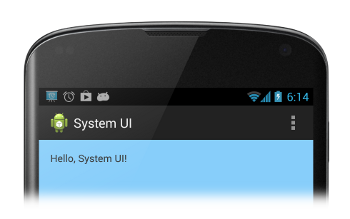
\includegraphics[scale=0.9]{Chapter3/status_bar_show.png}
		\caption{Shows a mock android application with the status bar open. The status bar is the black panel with the text "System UI" and the approve device information such as notification, signal, battery, ect. This image was taken from the "Hiding the Status Bar" tutorial created by the Android development team \cite{hide_status_bar}.}
		\label{fig:status_bar}
	}
\end{figure}


An additional task that was required alongside the creation of the welcome screen of the Android app was to remove the status bar from the Graphical User Interface (GUI). The status bar can be seen in Figure \ref{fig:status_bar} and the \textit{"Hiding the Status Bar"} tutorial \cite{hide_status_bar} from the Android developer site, gave an insight into how this could be removed from the app. When implementing the suggested changes from the tutorial, an error occurred routing from the call to the getActionBar() method that returns a pointer to the status bar. A stack overflow issue detailing this error \cite{sof_status_bar_err}, helped to diagnose the cause of the issue. The version of android being used was utilising the new
\begin{verbatim}
android.support.v7.app.ActionBarActivity
\end{verbatim}
which needed to be accessed as a support status bar rather than the older style regular status bar. This could be done using the function: 
\begin{verbatim}
getSupportActionBar()
\end{verbatim}

\subsection{UI testing}
To ensure that all elements of the Android application were subject to some form of automated testing, UI tests were developed for the Android app. These tests included checking page contents as well as page transitions to ensure that the expected content was visible and the buttons functioned correctly. As described in the Android developers guide \textit{"Testing Apps on Android"} \cite{testing_apps_on_android}, two types of test are commonly used for testing Android applications.

\begin{itemize}
	\item \textbf{Local unit tests}: Unit tests in this case are similar to any standard unit test for a normal code base. They test function input and output given various states. These tests are run on the local machine using the Java Virtual Machine (JVM) and have access to the Android specific API functions.
	
	\item \textbf{Instrumented tests}: By contrast, the Instrumented tests run on a hardware device or emulator. They are designed to test the app while it is running rather than testing individual functions, like a unit test. This allows for tests that exercise button transitions or page content to be run in an automated way.
\end{itemize}

For the UI testing, Instrumentation tests were developed and run on a mobile device attached to the development machine.

Whilst running tests for page content was straightforward, attempting to test page transitions proved more complex. A stack overflow issue was found that helped in to determine how this operation could be achieved \cite{sof_android_button_test}. The answer to the issue detailed using an ActivityMonitor class to listen for an Android Intent (the commands issued at the time of page transition) being executed.


\subsection{Background subtraction multi-threading}
Finally, this iteration revisited the background subtraction algorithm. Having already implemented the green screen algorithm, the algorithm or execution of the algorithm needed to be optimised to produce an acceptable frame rate. To do this, investigation in Python multi-threading took place. Each pixel in the input image needed to be checked and if it was above a certain value of green, changed to be black. This operation was performed on every pixel independently one after another. To improve the speed of execution, instead of checking the full array of the image in the main thread, the image was divided into 4 quadrants and each processed in a separate thread. Initially this was done in place in the array where each thread was given a start and end index to check. However, after implementing this solution, it was found to not have decreased the execution speed. This was the result of the array being locked while processing. To avoid multiple threads accessing the same NumPy array and potential corrupting the data, the array is locked while one thread accesses it meaning that the next thread must wait for the first to finish. 

By creating new array objects that relate to each quadrant the lock problem was avoided, however only a slight decrease in execution time was found. More detailed investigation revealed that this was caused by the time taken to initialise new arrays with the data from each quadrant.

Again, as no solution was found for execution time issue, development of the background subtraction algorithm was halted. Instead it was decided to use a black background when filming. Whilst this solution offers less versatility in the location where actors can be filmed, it means that the frame rate of the hologram remains close to that of the camera feed. 

  
\newpage

\section{Iteration 4}
\textbf{Date}: 13/03/2017 \\
\textbf{Features}: 6, 7, 8 \\
\textbf{Overview}: Aberystwyth University Science Week was scheduled to begin on the 14th March 2017 and last a duration of three days. All the work required for the prototype (Feature 1-4) had been completed or alternative solutions found, as such it was possible to take the prototype to the event to test it with the target audience. In addition, this iteration concluded with a demonstration of the project so far on Friday 17th March. 

\subsection{Aberystwyth Science Week 2017}

\begin{figure}[h!]
	\centering{
		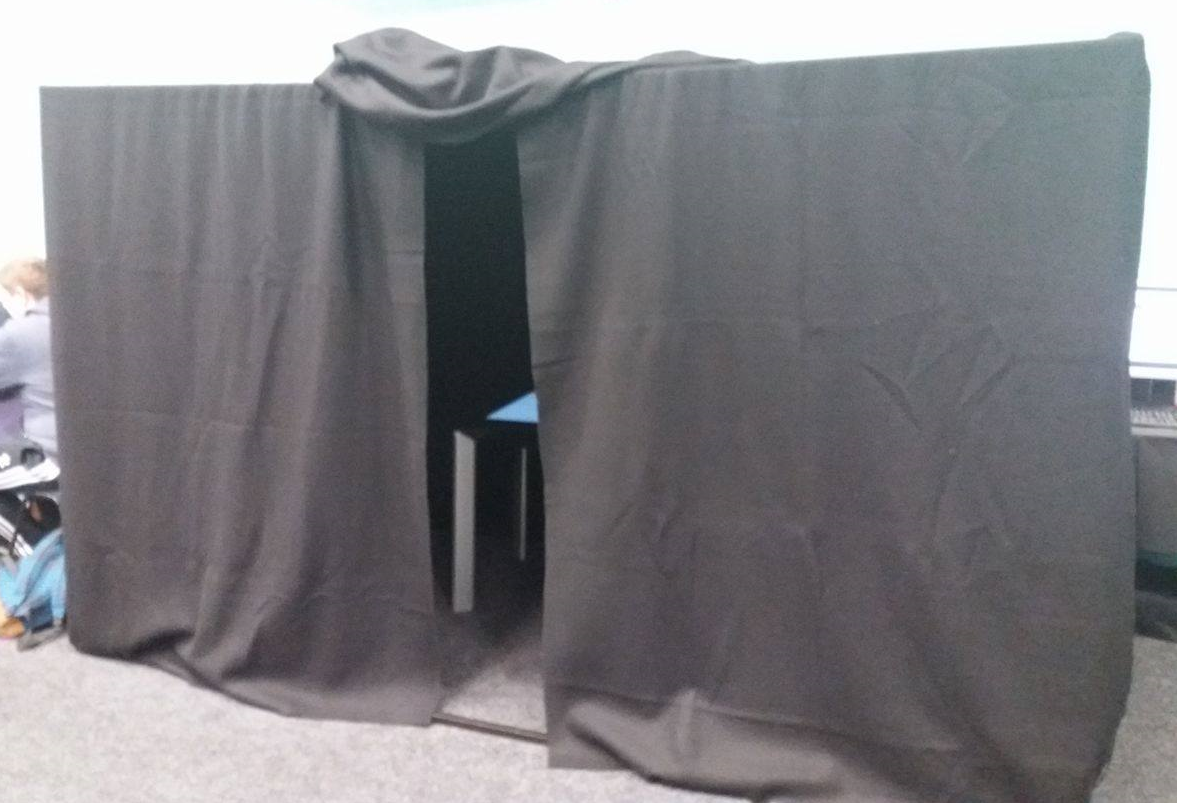
\includegraphics[scale=0.3]{Chapter3/viewing_area_science_week.png}
		\caption{Shows the viewing area for the real-time hologram creation system at the Aberystwyth University Science Week 2017. Inside, part of the touch screen table (being used as the display monitor for the system) is visible.}
		\label{fig:science_week_viewing_area}
	}
\end{figure}


The entities listed in the component diagram (the staging area, viewing area and image processing machine) were all constructed at the event venue. Figure \ref{fig:science_week_viewing_area} shows the viewing area (large black tent housing the monitor for the Pepper's Ghost Pyramid). To the right of the tent a camera attached to a computer was set up to record members of the audience. The camera was attached to the computer via a USB cable and the computer was attached to the external monitor in the tent via a HDMI cable.

Two main pieces of feedback could be inferred from using the prototype at the event. The first is that it proved a great success, with the clear majority of visiting students appearing greatly interested and engaged by the impactful display. The second was that students were not given much time at the event (most schools were present for an hour), meaning that the time that students were able to spend at each stall was limited. Originally, the Charades Game was designed to be played where actors and viewers would swap every time a correct answer was given, as would be the rules in a conventional game of charades. However, after discovering the limited time window for each activity at the science week, this concept was adjusted going forward to better suit the use case. To do this, two changes to the game rules were made:

\begin{itemize}
	 \item Actors act three phrases, and a points system was used, giving viewers points for correct guesses. At the end of each round, the viewer with the highest points would become the actor. This change enabled more time to be spent using the system, and less time for the member of the audience to be swapping roles.
	 
	 \item The subject of the phrase was changed to make more phrases single words and, rather than using conventional genres such as books and films, genres were changed to be activities and animals. These new genres meant a large amount of phrases were shorter and avoided long titles with simple words. A good example of where long titles would have been a problem is with the book "The Lion, the witch and the wardrobe". This phrase could take some time to act out fully due to the large number of words and it is also difficult to act simple words like "The".
\end{itemize} 

\subsection{Mid project demonstration and conclusions}
The mid project demonstration overall was a success and the demonstration of the software worked well. However, the question was raised as to why the charades system had been designed as an android application. The original reasoning for an android app was to promote the use of hand held devices for interaction with the system. Moreover, an Android app can potentially remove the reliance on the internet via the use of Bluetooth or locally connecting the devices together. This is an important factor to consider if, for example, an outreach event was being held in an area or building with poor reception. Furthermore, an android application removes problems that can occur with users attempting to manipulate the system via the URL which can be the case in some web apps.

Despite this, on re-evaluation of the project requirements and the final use case of the system, a web app was a better choice. The web app implementation removes many of the complications that could be faced with an android application which include:
\begin{itemize}
	\item Enabling devices to communicate with one another: Whilst there are many technologies for performing communications between android applications such as over the internet, via Bluetooth or through a peer-to-peer system, these technologies can be difficult to implement and test.
	\item Limiting the number of devices that are available: Whilst the event organisers would normally be able to get several tablets and mobile devices to use with the system. If users wished to join in on their own devices this would require that both the device they are using is on the android operating system, and the app is available on the Google Play Store.
\end{itemize}

A web app solves the above problems as it is already hosted on the internet which will allow for implicit communication between device accessing the system. Furthermore, the web app will be platform independent as the system code is executed server side and users interact with it through a web client.

This decision was difficult as due to the events of the week, little progress had been made on the android application. Starting again with a web application would mean further setbacks, but at the time the decision was made that it would lead to a better product.

\newpage

\section{Iteration 5}
\textbf{Date}: 20/03/2017 \\
\textbf{Features}: 9, 10 \\
\textbf{Roll-over features}: 5, 6, 7, 8 \\
\textbf{Overview}: This iterations first task was to adjust the features list schedule due to the decision to change to a web app from an Android app. Therefore, this iteration dealt with the roll over issues from the previous iterations, and Feature 9 and 10 (which were originally planned for this iteration) were redistributed among future iterations.

\subsection{Django}
As the hologram creation software already used the Python programming language, it was logical to use a Python framework for implementation of the website. Several Python web framework exist with the most popular being Django, Flask and Pyramid. The article \textit{"Django vs Flask vs Pyramid: Choosing a Python Web Framework"} written by Ryan Brown \cite{python_webframework_comparison}, was a useful resource in making a decision regarding the best framework to use. In the Article, Django is identified as the most popular of the three as well as being best suited to mid scale projects like the Charades system. Furthermore, Django uses to many familiar keywords and concepts to those ruby on rails which is a technology that the developer had used prior. Finally, an excellent tutorial for the Django web framework by Nigel George, \textit{"Masting Django: Core"} \cite{django_book} is available for free online. 

\subsection{Model}
As described in \textit{"Mastering Django: Core} \cite{django_book}, the initial web site set up was fast and straightforward. This process was made simpler by not having any requirement for a database and having models written as Python classes. However, using Python class meant that there was an additional requirement for tests to ensure the model functioned correctly. This would not have been required of a database as they are tested by the database supplier (for example SQL) before release. The tests for the Python class models were written as Python unit tests. As the model did not rely on the Django web framework, classes could be considered independent from the rest of the system and tested in isolation.

The model can be found in the directory ...

\subsection{Template}
The templates in Django are written in html and can use embedded Python code to execute additional commands or access variables. The variables are pushed to the template through the controller and can then be accessed by surround them in double curly brackets:
\begin{verbatim}
{{ variable_name }}
\end{verbatim}

Embedding python code also proved powerful for flow control and conditional statements. An example of both of these being used can be found in Appendix C section \textit{Embedded Python}.

The template code can be found in the charades\/templates directory.

\subsection{View}
The view code is the controller for the website and acts as the link between the model (data) and the template (what is shown to the client). The views.py file is where this code is stored and consists of multiple view functions. The view functions must have an input of a request (which is a HTTP request header) and must return a the request along with some rendered data (the template code). It is at the point where the request is returned that additional data can be provided to the template in the form of a python dictionary.

The HTTP request is handled by the urls.py file which holds the routing information between the URL and the controller. Figure \ref{fig:django_routing} visually represents how these interactions take place.

The view code can be found in the charades\/charades\/views.py file.

\begin{figure}[h!]
	\centering{
		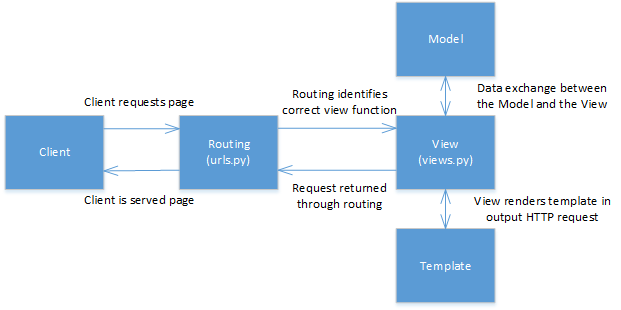
\includegraphics[scale=0.3]{Chapter3/django_routing.png}
		\caption{Show the interactions between the client, the urls.py (routing) file, the template, the view and the model in the Django web framework.}
		\label{fig:django_routing}
	}
\end{figure}


\newpage

\section{Iteration 6}
\textbf{Date}: 27/03/2017 \\
\textbf{Features}: 9, 10, 11 \\
\textbf{Overview}: This iteration covered access and security for the Charades Game and dealt with functions to ensure that only those at an event would be able to log on. Furthermore, to improve the security of malicious users, redirects were put in place to stop access to certain pages depending on the game state.

\subsection{Session password}
To disable access from those outside an event (such as the Aberystwyth Science Week), a session password was added to the landing page of the website. When a user chooses a type (actor or viewer), they are also required to provide the session password to access the system. By default the session password is stored in the view code as \textit{"BSW18"} but this can be changed easily. If mobile devices capable of accessing the system were provided for an event where the system was in use, the organisers would be able to type in the session password before the arrival of any visitors. Alternatively, (if guests were to use their own devices) the session password could be displayed on a sign at near the viewing area enabling users to log in themselves.

\subsection{Cookies}
When a valid session password has been provided, the password is then stored client side in a cookie. The Django online documentation \cite{django_cookies} provided a tutorial which aided greatly in the implementation of a session cookie. on implementing  In addition, the cookie also stores the type of user (actor or viewer) and, if the user is a viewer, the unique number used to identify them. This unique number is called the viewer\_number and is generated by the system when a new viewer joins. The number can then be used to lookup the viewers score:

\begin{verbatim}
	viewer_number = request.session['viewer_number']
	...
	viewer = GAME.lookup_viewer(viewer_number)
	points = viewer.points
\end{verbatim}

The above code is from the waiting\_for\_actor function in the \/charades\/charades\/views.py file. The above code returns the current score of the viewer accessing the waiting\_for\_actor.html page. The code first finds the viewer number from the session variable (cookie), and then calls the lookup\_viewer function in the Game class, using the viewer\_number as input. This will return the Viewer object relating to the viewer\_number provided. Finally this object can be used to see how many points the user has accumulated.

\subsection{Redirects}
\subsubsection{State based redirects}
Each page of the website (excluding the landing page) queries a part of the model. It is possible that, without proper handling, either intentionally or not, a user can access a page that the system state does not yet allow for. An example of this is if a viewer attempted to access the guess.html page (where they are asked to guess the current word or phrase) before the actor has chosen a phrase. Accessing this page at this time could cause errors to be thrown and potentially corrupt the game state. To stop this from happening, state based redirects have been added to the website controller. These are functions that, instead of returning the page content that would normally be provided from the requested URL, redirect the user to a different URL. The different URL will then handle the request appropriately. In the above case of accessing the guess.html page before it is ready, the viewer will be redirected to the instructions page which displays a "Please wait" message as shown in Figure ... .

** ADD FIGURE FOR REDIRECT ON GUESS.HTML ** 

\subsubsection{User type redirects}
Similarly, users can attempt to access webpages that are only designed for a different type of user. An example of this is that the phrase\_selection.html page is designed for the actor to select a phrase to be acted. Once selected this data is then passed to the model and the viewers are able to guess the word or phrase. It should not be possible for a viewer to access the select\_phrase.html at any time, therefore user type redirects have been added to the controller to ensure this is not possible. The user type redirects are designed to check the type of user attempting to access the content by searching for the 'user\_type' entry in the session variable. If the incorrect user\_type, or no user\_type at all, is found in the session variable, the client will be redirected to the landing page, and an error message will be displayed as shown in Figure ... .

** ADD FIGURE FOR REDIRECT ON YOU'RE NOT AN ACTOR **
\newpage

\section{Iteration 7}
\textbf{Date}: 03/04/2017 \\
\textbf{Features}: 12, 13, 14 \\
\textbf{Overview}:

\subsection{Real time updates}
The charades game has multiple users logged in at the same time and has several scenarios where interactions need to take place in real-time. An example of a real time interaction, is that when a phrase is guessed correctly by a viewer, the actor must be informed and prompted to select a different word.

When the Django framework was created, it was designed to handle static website that were more common of those seen 5 or 10 years ago. In this respect, at its core Django is built around answering requests from the client, but does not have any methods to push data to the client by default. However, many technologies provide solutions to real time communications for the web and can be implemented in Django. The approach chosen for this project was to use an API and a polling system to mimic the pushing of data from the server side to the client. 

An alternative consideration was made to use the new Django Channels technology. Django Channels provide a way to opening a bi-directional connection between the server and the client, allowing data to be pushed both ways (client to server and server to client)\cite{django_channels}. This technology utilises the new WebSocket protocol. Whilst this technology would provide a solution to the aforementioned problem, implementing the technology is a complex tasks than a polling system. It is however and better and more long term solution but the additional time it would have taken to implement would have set the project back further.

\subsection{API}
An Application Programming Interface (API) was created as a way to programmatically assess the current state of the system. As with any Django page, when a request is sent from a client (for example the user types the page URL into the address bar) the page is loaded and any data that is embedded in the template will be updated automatically. In the case of an API, simple data that represents a fact in the system can be displayed. In the case of phrase\_ready.html, this page, when loaded, is given data from the controller. The controller function (See Appendix C, Section \textit{phrase\_ready API}) checks the current state of the system, and produces a True or False value as to whether the phrase is in a guessable state. The state of the system will change depending on the user interaction with the system. For example, if a phrase has not yet been selected by the actor, the phrase\_ready API will display False. Once a phrase has been selected, the controller will receive the data from the client request, update the current phrase in the system and then, when the API is polled (loaded) it will have the new value of True.

\subsection{Polling}
As Django does not provide a built in methods of pushing data to the client (as discussed above), the client most poll the API to establish if the state of the system has changed. This is done using the JavaScript setInterval() function \cite{js_setinterval}. This function takes a parameter of another function and a time interval given in milliseconds. When that number of milliseconds has passed, the provided function will be executed. To poll the API the project used a function that was designed to retrieve information from the API pages using an HTTP GET request. This function (detailed in Appendix C, section \textit{Polling function}) was the primary input to the set interval function. When the data is received from the API, conditional statements within the function decide what should happen. In most cases this is a page refresh and then the controller will supply new data to the page.

Depending on the polling function, the API is normally polled every second with some cases having larger polling intervals if  an instantaneous answer is not required. This method of communication does have one small caveat, if two users were to guess the word within one second of each other, it is possible that both viewers would receive points. The reason for this interaction is that when a viewer guesses a phrase correctly, the API is updated and then all the viewers (on the guess.html page) are redirected to the waiting\_for\_actor.html page. During the time the other viewers are polling the API it is possible that a guess could still be submitted and, if correct, the controller would increment the score of the viewer who guessed correctly. This would result in the above interaction where two or more player potentially score points if they guess within a second of each other. Statistically, a full second window for another viewer to guess is the worst case scenario as it is likely that a viewer makes a correct guess mid way through a polling cycle. This would result in a 0.5 second window which was deemed acceptable.

\newpage

\section{Iteration 8}
\textbf{Date}: 10/04/2017 \\
\textbf{Features}: 15, 17 \\
\textbf{Overview}: The final iteration covered two main tasks. The first was to decide on a end game condition and scoring, and the second to perform some refactoring of the of the Charades Game to improve readability and maintainability.

\subsection{End game conditions and scoring}
In order to ensure that the game was completed in a timely manor and the outcome was fair the scoring system and rules had to be decided upon. The rules, as previously mentioned were changed to include a scoring system as well as multiple rounds. The game lasts for a duration of three rounds, where a round is a single phrase being guessed. Although the main purpose of the game is to be an aid to showcase the hologram system, for the younger target audience, having a friendly competition would prove more interesting for them. The phrase dictionary consists one or two word phrases, as such the whole phrase is worth 20 points, and a single word is worth 10. At the end of a round a new actor is chosen based on either a volunteer on the highest scoring viewer.

\subsection{Refactoring}
The controller (views.py) for the Charades Game had been continually added to throughout the development period. It contained all the functions for executing control code in a single file, and had some code duplication. To improve this, the code was refactored to firstly ensure that duplicated code was removed and secondly to make the controller easy to read. This was an important step as, providing this system would be used in the future, it would most likely require adaptation to remain current. Refactoring the code base also gave the advantage of allowing more tests to be added to the simpler helper functions which improved the overall test coverage of the system.

\newpage

\section{Implementation review}
You can conclude this section by reviewing the end of the implementation stage against the planned requirements. 
\chapter{Testing}

The project requirements state \textit{"Given the target audience, the system should be robust and difficult to crash."} In order to achieve this, testing should be a priority to ensure a functional system. Furthermore, the testing of this project (as proven below) is comprehensive and attempt to cover all eventualities. With a combination of automated, manual and user testing, a reasonable degree of confidence can be stated with regards to the robustness of the project. 

Whilst data security did not need to be considered for this project (as no sensitive data is stored) security against cyber attacks and malicious use have been considered through out the testing and development process. For the most part, Manual testing has been used to uncover potential flaws in the security of the website and when discovered, additional automated tests have been added to safeguard against these issues in the future.

\section{Overall Approach to Testing}
The project used TDD as part of the process for software implementation. As well as designing features, tests were also designed for the required functions before functional code was written. There were two main types of tests for the website: unit tests, that test the functionality of the model and the controllers, and system tests, that use selenium to check the flow of the system and simulate the actions of a user. Where appropriate, tests for functions were written to test three different cases:

\begin{itemize}
\item Success case: Simulates either an expected input parameter for the function or an expected state that the system should be to run a function.

\item Edge case: Checks the maximum functional range of the functions input parameters. For example if the function was only designed to allow 5 viewers to participate in a game, then it would check that the when the viewers total 5 the function still passes.

\item Failure case: Ensures that given incorrect parameters or system state, the function will fail in the expected way.

\end{itemize}

An example function and corresponding test cases displaying the above approach to testing can be found in Appendix C, section (...).

For unit tests, tests were organised into classes were each test class would test a class or module of code. Similarly, system tests were designed to test a single Django template. The requirement for adding code to the master branch is that all unit and system tests (past and present) must pass and the static analysis tools must produce no errors.

\section{Automated Testing}
\subsection{Jenkins}
To improve the consistency of the code base, the GitHub repository was linked to a local Jenkins server. This server was set up at the beginning of the project and was used as part of the development life cycle of each feature. The Jenkins server ran as a background process on the development machine. The set up for the Jenkins server followed two guides: The official Jenkins Windows Service installation guide \textit{"Installing Jenkins as a Windows Service"} \cite{jenkins_wiki_install} from the Jenkins.io wiki and Steve's Blog \textit{"Automated python unit testing, code coverage and code quality analysis with Jenkins"} \cite{steves_blog} a self hosted technical blog from a software developing consultant specialising in Python.

Whilst Jenkins offers the ability to run tests periodically, this feature was not used and tests were triggered manually by the developer. The reasoning behind this is that incremental time based builds were not required. Had the project been developed by a team, the need for timed builds is more justifiable as many developers will be pushing code changes simultaneously. In a single person developer team, code is pushed one feature at a time and the work flow is linear hence there is no justifiable requirement for periodical builds. Despite this, the use of Jenkins is still admissible in a single developer project as it allows for centralised building of the project in a controlled, repeatable, environment. Additionally, The formatting for results produced by Jenkins offers an easy way to quickly visualise problems with the code base.

\subsection{Static analysis}
\subsubsection{Pylint}
Pylint is a linting tool that follows the PEP8 standards \cite{pep8} for python coding. The linter runs static analysis on the code base and ensures that all code meets with the standards specified by PEP8 (and produces warning and errors were this is not the case. The PEP8 standards include guidelines style and syntax as well as documentation (in the form of doc strings). Whilst several standards for the Python coding language are available, PEP8 was chosen as it is promoted by the developers of the Python language and is the most popular. An example of the Pylint output rendered by Jenkins is displayed below in Figure \ref{fig:jenkins_pylint}. In this Figure, the peak correspond to when pull request are initially pushed to Jenkins and troughs are were the Pylint warnings have been resolved.
\begin{figure}[h!]
	\centering{
		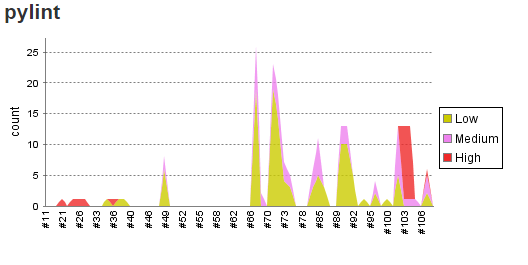
\includegraphics[scale=0.75]{Chapter4/jenkins_pylint.PNG}
		\caption{The output of the Pylint test run on the full code base rendered by Jenkins. Here, the number of warnings, and there severity, is logged by each build number.}
		\label{fig:jenkins_pylint}
	}
\end{figure}

\newpage

\subsubsection{Test coverage} 
An additional testing package, nosetest \cite{nosetest}, was used to run python tests for this project. This package, amongst other advantages, produces reports that are interpretable by Jenkins for both unit tests and test coverage. As the web based charades game was written in Django (which has its own testing framework), nosetest could only be used for the hologram creation software. The test coverage displays graphically the proportion of the code that is run in tests. Although basic, this helps to highlight potential conditional statements, function and even lines that are not being tested. 

An example of the test coverage output rendered by Jenkins is displayed below in Figure \ref{fig:jenkins_test_cover}. Figure \ref{fig:jenkins_test_cover} shows that whilst the majority of the code base is covered by testing, several lines are excluded. These lines had to be omitted from tests as their functionality was to the perform the video processing loop. Whilst the functions that are called within that loop are sufficiently tested, the loop itself can not be tested easily as it creates an output window. The output window is only successfully closed via mouse click on the window close button (an operation not easily replicated in tests).
\begin{figure}[h!]
	\centering{
		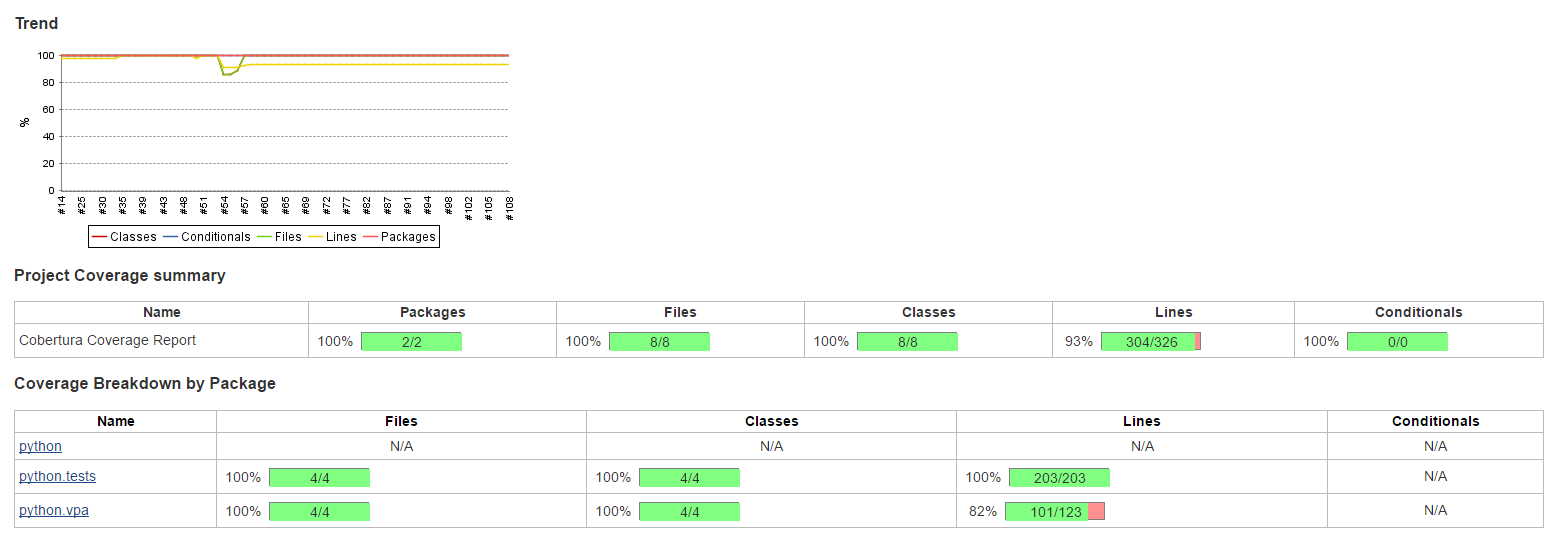
\includegraphics[scale=0.75]{Chapter4/jenkins_test_coverage.PNG}
		\caption{The rendered output of the test coverage report from nosetest in Jenkins. Note the incomplete test coverage (for lines) and see explanation in section 4.2.2.2.}
		\label{fig:jenkins_test_cover}
	}
\end{figure}
 

\subsection{Unit Tests}
To ensure the functionality of the system, unit tests were created to test functions. The unit tests were written using the python unit test framework provided by the python language \cite{python_unittest}. The unit tests are designed to be atom and test a single part of functionality per test. As such, more complex functions that dependant on the state of the system or have multiple return values will have multiple test associated with them designed to exercise every line of the code. Unit tests were written in classes where one class will test only one python class or module.

The tests for the hologram creation software are stored in a different directory to the source code. Python's solution to this is to import the source code modules from the other directory so they can be used in the test cases. This however, is only possible if the shared parent directory of both tests and source code is a python module itself. If this is not the case, a context file should be used to mitigate the issue. The context file (Appendix C, section ...) is used to import the module by first setting the correct directory path for python to be able to find it. This context file is ten import itself at the start of every test.

Figure \ref{fig:jenkins_unit_test} shows the graph created by Jenkins and nosetest that represents the pass and failure state of each unit test for every build. The graph shows an upwards tread as the number of tests being run in the project increase with the creation of additional issues. To be accepted into the master branch of the GitHub repository, all tests must pass.

\begin{figure}[h!]
	\centering{
		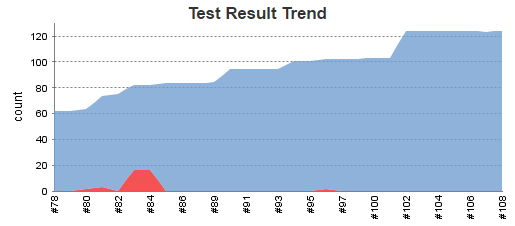
\includegraphics[scale=0.75]{Chapter4/jenkins_unit_test.PNG}
		\caption{The rendered output of the unit test report in Jenkins. Blue indicates passing tests while red is those that failed.}
		\label{fig:jenkins_unit_test}
	}
\end{figure}

\subsection{User Interface Testing}
The Python Selenium module,  was used for all the testing of the user interface. The selenium library allows for interaction with a web browser in a testing environment. The common actions that can be performed programmatically include button clicks, filling in text fields and changing the current URL of the page. All user interface tests have several generic tests which are as follows:
\begin{itemize}
	\item Page elements: The generic view of a page is tested to ensure that the elements on the page are what the test expects. This is mainly used as a test of the Django template code, written in HTML, and the embedded Python.
	\item Navigation: Most pages of the website will either have a button to take the user to another page, or poll the api until the conditions are met to redirect the user. In both cases, a test case will exist to ensure the page transition is correct. 
\end{itemize}
In addition to these tests, the website had to be tested to ensure that the URL could not be manually changed to affect the state of the game. An example of this would be attempting to visit the phrase\_selection.html page (where the actor selects a phrase) as a viewer.  In a scenario like this, the user is redirected to the index page with an error message display and this is also tested as part of the user interface testing.

\subsubsection{Selenium start up time}
Selenium gives the advantage of being able to test a web interface. However, when run locally, selenium took on average 6 to 8 seconds to create a new instance of a web browser. For continuity between tests,  much of the online documentation that was used in this project, such as \textit{"Selenium with Python : Using Selenium to write tests"} \cite{selenium_guide}, proposed running a new instance of the selenium web driver for each test. The reason for doing this is that it will restart the web browser and remove any cached data or session information. However, with a growing number of selenium test, the time taken to run the full test suite was no longer practical.

To remedy this, the change was made to use only one selenium browser per class of tests \cite{django_live_server_test}. The selenium instance was initialised in the class setUp function and closed in the class tearDown and then the cached data was manually removed from the web browser instance. Whilst this does leave scope for having some cached data remain in the web browser between tests, this reduced the number of web browser reinitialisations to be equal to the number of test classes (8) from the number of tests (27) hence saving a third of the time when executing the tests.

\subsubsection{Using selenium with Django and Localhost}
During the development of the project the website was hosted on the local development machine using local host. In order to test the website with selenium, a hosted version of the website must be accessible. For manual developer testing, Django offers the ability to run a server locally and host the website using the command: \begin{verbatim}
python manage.py runserver 
\end{verbatim}
to run the start the server. The website is then accessible from http://localhost:8080 (by default). To allow selenium tests to run successfully, a method of starting the server before tests were run needed to be discovered.

The original way of doing this was to run the above command to start the server before tests were run. Whilst this does resolve the problem, it forces the tests to be reliant on the correct port (default 8080) being used to access the website. This port can be specified upon starting the server, but this could produce conflicts in different development environments if, for example, the development machine had other services running on the same local port.

A more permanent solution was discovered in the Django documentation \cite{django_live_server_test}. This section of the documentation described the use of extending the StaticLiveServerTestCase rather than extending python UnitTest. The extra functionality provided by extending this module means that when the test class is run, it launches a live Django server to host the Django web content stored in the same project. This service defaults to running on localhost:8081, but the full URL is accessible during test execution with the python code:
\begin{verbatim}
self.live_server_url
\end{verbatim}
This above code returns a string value that matches the correct port address on localhost to where the server is running. Using the LiveServerTestCase resolves both problems mentioned above as firstly, there is no longer a need to hard code the url including the port number and secondly, the server exists only for the life span of the test meaning there is no need to start a separate server manually before the tests are executed.

\section{Manual Testing}
\subsection{Charades Game}
In addition to testing the web site code with automated unit tests during most features, a manual test performed by the developer was carried out. The manual testing was designed to be a supplementary testing phase to ensure that functionality was correct and no exceptions or errors are raised unexpectedly. In the case that problems were discovered, these issues would be written as a formal test case and added to the test classes to ensure the functionality is checked in the future. The Manual testing followed multiple patterns of use.
\begin{itemize}
	\item Normal user workflow: The expected user workflow is followed to ensure that a typical user performing valid, and expected, operations causes the expected behaviour with no failures.
	
	\item Unexpected behaviour: Users will not always follow the expected workflow of the website and can occasionally enter values incorrectly. This testing was performed on new features user interfaces and ensured:
	\begin{itemize}
		\item No invalid entries could be put into text or number entry fields.
		\item Submitting test fields in forms does not produce errors. 
		\item Pressing the back button on a web page does not cause errors for either the user or the system.
	\end{itemize}
	
	\item Malicious behaviour: Tests were carried out to ensure that the website could not be compromised deliberately by a user. Some of the information passing in this website uses the HTTP GET protocol and subsequently, that information is stored in the client side URL. It is possible that a user with malicious intentions may attempt to taint the information provided in the URL to corrupt the system. As such, test were carried out to ensure that information in the URL was sanitised and expected.
\end{itemize}


\subsection{Hologram creation program}
Manual testing was carried out a smaller scale for the hologram creation program. As discussed in section 4.2.2.2, several lines of code within the main display loop could not be unit tested. To ensure the functionality of this code, manual testing was performed to ensure correct functionality. This was the only manual testing performed on the hologram creation program as there was no user input and output required.


\section{User Testing}
User testing took place at the Aberystwyth Science week event in March 2017. The event lasted for three days and gave the opportunity to test the prototype of the hologram system with the target audience. A black tent was set up in the event hall and this housed the touch screen table being used as an external monitor for the holographic display. The web cam for the video feed input was set up outside the tent and used to record viewers. When new viewers entered the viewing area, initially a test video would be running and then, after explaining the technique, audience members were given the opportunity to be filmed to create a hologram that was displayed to their peers.

\subsection{General findings}
The stall at the event generated much intrigue amongst the audience. Many thoroughly enjoyed seeing their peers project holographically, but there was a clear lack of purpose for those being filmed other than waving to a camera. This helped to confirm the need for the charades system to be used alongside the hologram creation system.

\subsection{Limited time}
Given the events size, the number of stalls and the limited time that each visiting school had at the event, a new consideration needed to be made regarding the amount of time required to play the game. Whilst the initial idea had been to swap users who were acting after every correct guess, this would invest a lot of the time that users had at the stall with swapping players rather than playing the game. To accommodate for this, the game flow was amended to have 3 phrases acted by the same actor and points accumulated by the viewers.

\subsection{Camera distance}
The charades game will require the actors whole body to be visible on camera while they are acting. At the event only the head of the actor was filmed using a standard web cam. Whilst this was in part because there was no advantage to filming the rest of the body given the state of the prototype, this was affected by the amount of space in the event hall. To resolve this issue at the next event, a wide angle camera orientated vertically would allow for a larger amount of the body to be filmed in same amount of space. However, this approach may require adaptations of the hologram creation software to avoid over cropping the video feed.
\chapter{Evaluation}

\section{Methodology}
Choosing FDD for the project proved useful from a structural and time management perspective. Whilst multiple adaptation needed to be made to ensure the methodology was suitable for a single developer, the adapted methodology still capture the core concepts of the original specification. Developing features one at a time and having a set work flow for developing those features, helped to schedule tasks, and avoid being overwhelmed by the scale of the project. In addition, as FDD provided an upfront design phase it was far easier to obtain insight into the size of the project, as well as identifying areas that would take longer to implement.

Whilst the methodology was a success overall, it could have been further improved with additional adaptations. Originally, it was planned that pull request would be left open on GitHub for a day, before they were reviewed to check for code quality. This in principal was a good idea but caused problems due to the dependencies between features. The feature list details that almost all features are dependent on the previous feature being complete. As such, delaying the code review for a day would cause a delay in development. This problem could have been resolved however by developing the charades system and the hologram system in tandem. By doing this, it would have been possible to leave time to review one systems code while writing the other (hence not losing any development time).

\section{Requirements identification}

Since the initial creation of the objectives stated in chapter 1 section 1.4.1, some additional considerations have been added. Firstly, there is no mention of security explicitly in the objectives. The justification for this is that neither system produced in this project stores any personal data. Therefore, from a data security aspect, there is no requirement to protect user data. However, there is other security aspects to consider such as SQL injection or Cross-Site Request Forgery (CSRF). These forms of security threat have been addressed in the project although not stated in the objectives and in hind sight, it would have been better to have security explicitly stated as a requirement.

An additional objective that was not stated and should have been added was to ensure that the Charades Game UI was mobile compatible. The system itself was developed on a 17.3" monitor but rarely checked for how it would appear on a smaller (mobile) device. This would be an area of improvement that could have be made going forward and would greatly benefit the users. By using an adaptive design based on screen size, it would be possible to have a display that would be correct for any size device.

Aside from the above statements, the requirements for the project were well written and helped to focus the project and ensure it did not go out of scope. All the project objectives that were set have been addressed in some way in the project. This system has been well written and has a very high test coverage, which suggests that the system is very robust. The software includes error checking at runtime (in the form of input parsers), as well as logical checks to ensure that any user input is valid and expected. The robustness of this system was confirmed at the Aberystwyth University Science Week 2017, where the system functioned without error for the duration of the event.


\section{Design decisions}

The Charades Game was originally designed as an android application as discussed in the implementation section. This design decision was made due to language and technology familiarity for the developer. After further analysis, during the implementation of the project, the decision to switch to a web based implementation was made. This initially resulted in the loss of two weeks' work as the Android application so far had to be deleted. This decision was overall a positive change, but did potentially lower the quality of the software due to the time that was lost.

Neither the Android application or web application had a full design for the solution to communications. As this technology was relatively unknown to the developer, it was difficult the best method for implementation. Subsequently the communications design was vague. With more investigation into possible technologies for communication in the earlier stages of design, it would have been easier to make a more informed choice of the type of technology to use.

The design diagrams used to inform the overall model (section 2.1) proved very useful in helping to define the system. All the diagrams provided good insight into the requirements and structure of the system and were used throughout to help meet those requirements. Starting with a use case diagram helped to view the system at a very basic level of interaction. It helped to formalise all the operations that would be required of the system and ensured that no functional requirements were missed.

Creating UI designs helped to ensure that functions identified from the Use Case diagram were met. However, the diagrams could have been improved to help with system interaction. Being planned for use at outreach events, the system had to be designed with a young target audience in mind. In this respect, the UI design falls slightly short as the colour scheme could be more vibrant and enticing, and the interactions could have been designed in a way where instructions (displayed on the user and actor landing pages) are not required. Having not been able to test this system with the target audience, it is hard to establish if this is an effective UI.

\section{Use of Tools}
When the hologram system was being developed, it used the notepad++ text editor as the main editor for Python coding. However, when development of the Charades Game began, it required a better IDE that could help when developing code. The PyCharm IDE proved very helpful while developing the Charades System and on reflection would have been an excellent tool to use for development of the hologram system as well. Whilst it is unlikely that this would have further improved the code quality beyond its current state, it would have reached the state faster.

Throughout the project, Git and GitHub was utilised well making it easy to track progress, and organise features. The extensive use of Git along with sensible commit messages and correct issue number referencing made it easy to look back and see what development had been completed already. Furthermore, the use of GitHub templates for issue and pull request creation meant that a check list was already generated for each issue a pull request which contained the tasks to be completed. Although GitHub was an asset to the project, the way in which it was used, at times, was excessive and could get in the way of development. The GitHub workflow catered towards a team slightly more so than an individual. This meant that unnecessary tasks like assigning a developer to an issue or pull request had to be performed despite there only being one developer. Despite this however, Git and GitHub were an invaluable tool for version control, organisation, and backup throughout the project. 

Jenkins was used as an environment to run the automated tests for the system as well as perform static analysis. Using a service like Jenkins helped to regulate the test environment and produce an easy to comprehend output. The decision to use Jenkins as the CI tool of choice was made due to past familiarity with the service, however, on reflection, this could have been done locally just as easily. Jenkins has many features that were not utilised in this project such as project builds. Project builds is a tool that creates a build copy of the software after a set of tests have been run in the pipeline - which can be a useful output for manual testing. As this project was written in Python, there was no build output (as Python does not require compiling in a similar way to other languages such as C). Project builds is just one example of how Jenkins could be considered a heavy weight solution to having a controlled testing environment. Whilst it was a success in this project, it could be replaced by a light weight alternative should the project continue.

\newpage

\section{Improvements}
Keeping a diary throughout the project proved an invaluable resource when writing the report. The dairy helped with managing when development took place, the problems that were discovered and references that needed to be added. Were the project completed again, improving the diary even further would be an asset. As well as writing short bullet points that summarise issues that were dealt with that day, it would have been better to write a small paragraph. These paragraphs could then be used in the report to replace the overview at the start of the iteration. Furthermore, it would be better to reference features by name in the diary so that it can be more easily read without having to reference another document.

To obtain feedback on and improve the UI design, copies of the design could have been taken to the Aberystwyth University Science Week 2017. This would have given the opportunity to see if the target audience liked the design of the UI and what, if anything they might change. Collating these results then could have led to a better design that would be more fitting of the target audience.


\section{Future work}
There are many sections of the project that still require refactoring. Where this has been done already, the code is of very good standard, but sections of the Charades Game are not written as well as they could be. The main place where this is present is in the views.py file. This file holds all the controller functions for every page (including the API) and could quite easily be simplified through refactoring. The stages that would be done for this include, removing duplicate code used in redirects, moving simple code to other functions for both readability and maintainability, and using multiple files instead of just one to hold all the controller functionality.

An idea for a possible piece of future work is to enable the Charades Game and the Hologram creation system to interact with one another. The design for this would turn the camera (pointed at the actor) on when they were acting, and then display messages when either the actor is choosing a new word or phrase, or a viewer has guessed correctly. This could easily be done providing the hologram creation system and the Charades Game server are hosted on the same machine. The hologram creation system could poll a file on the machines hard drive, which contains what the hologram should currently be displaying (e.g. "Camera", "Winner", "Waiting"). The website would then be able to update the file when the game state changes.  

Currently the website for the Charades Game is not hosted anywhere online. Deploying this system to either a cloud service or on a server would not be a difficult task. The website can be installed and run using the installation instructions bundled with the project in the README.txt file. This would need to be done to use the charades system at future outreach events.

% add any additional chapters here

\setemptyheader
\addcontentsline{toc}{chapter}{Appendices}
\chapter*{Appendices}

% start the appendix - sets up different numbering
\fancypagestyle{plain}{%
%\fancyhf{} % clear all header and footer fields
\fancyhead[L]{\textsl{Appendix\ \thechapter}}
\fancyhead[R]{\textsl{\leftmark}}}

\appendix
\fancyhead[L]{\textsl{Appendix\ \thechapter}}
\fancyhead[R]{\textsl{\leftmark}}
\fancyhead[C]{}
\fancyfoot[C]{\thepage}
\renewcommand{\headrulewidth}{0.4pt}
\renewcommand{\chaptermark}[1]{\markboth{#1}{}}

\appendix
\fancyhead[L]{\textsl{Appendix\ \thechapter}}
\fancyhead[R]{\textsl{\leftmark}}
\fancyhead[C]{}
\fancyfoot[C]{\thepage}
\renewcommand{\headrulewidth}{0.4pt}
\renewcommand{\chaptermark}[1]{\markboth{#1}{}}

\fancyhead[L]{\textsl{Appendix\ \thechapter}}
\fancyhead[R]{\textsl{\leftmark}}
\fancyfoot[C]{{\thepage} of \pageref{LastPage}}

% include any appendices here
\chapter{Third-Party Code and Libraries}

If you have made use of any third party code or software libraries, i.e. any code that you have not designed and written yourself, then you must include this appendix. 

As has been said in lectures, it is acceptable and likely that you will make use of third-party code and software libraries. If third party code or libraries are used, your work will build on that to produce notable new work. The key requirement is that we understand what is your original work and what work is based on that of other people. 

Therefore, you need to clearly state what you have used and where the original material can be found. Also, if you have made any changes to the original versions, you must explain what you have changed. 

As an example, you might include a definition such as: 

Apache POI library - The project has been used to read and write Microsoft Excel files (XLS) as part of the interaction with the client's existing system for processing data. Version 3.10-FINAL was used. The library is open source and it is available from the Apache Software Foundation 
apache\_poi. The library is released using the Apache License 
apache\_license. This library was used without modification. 

\chapter{Ethics Submission}

Application Number: 6775

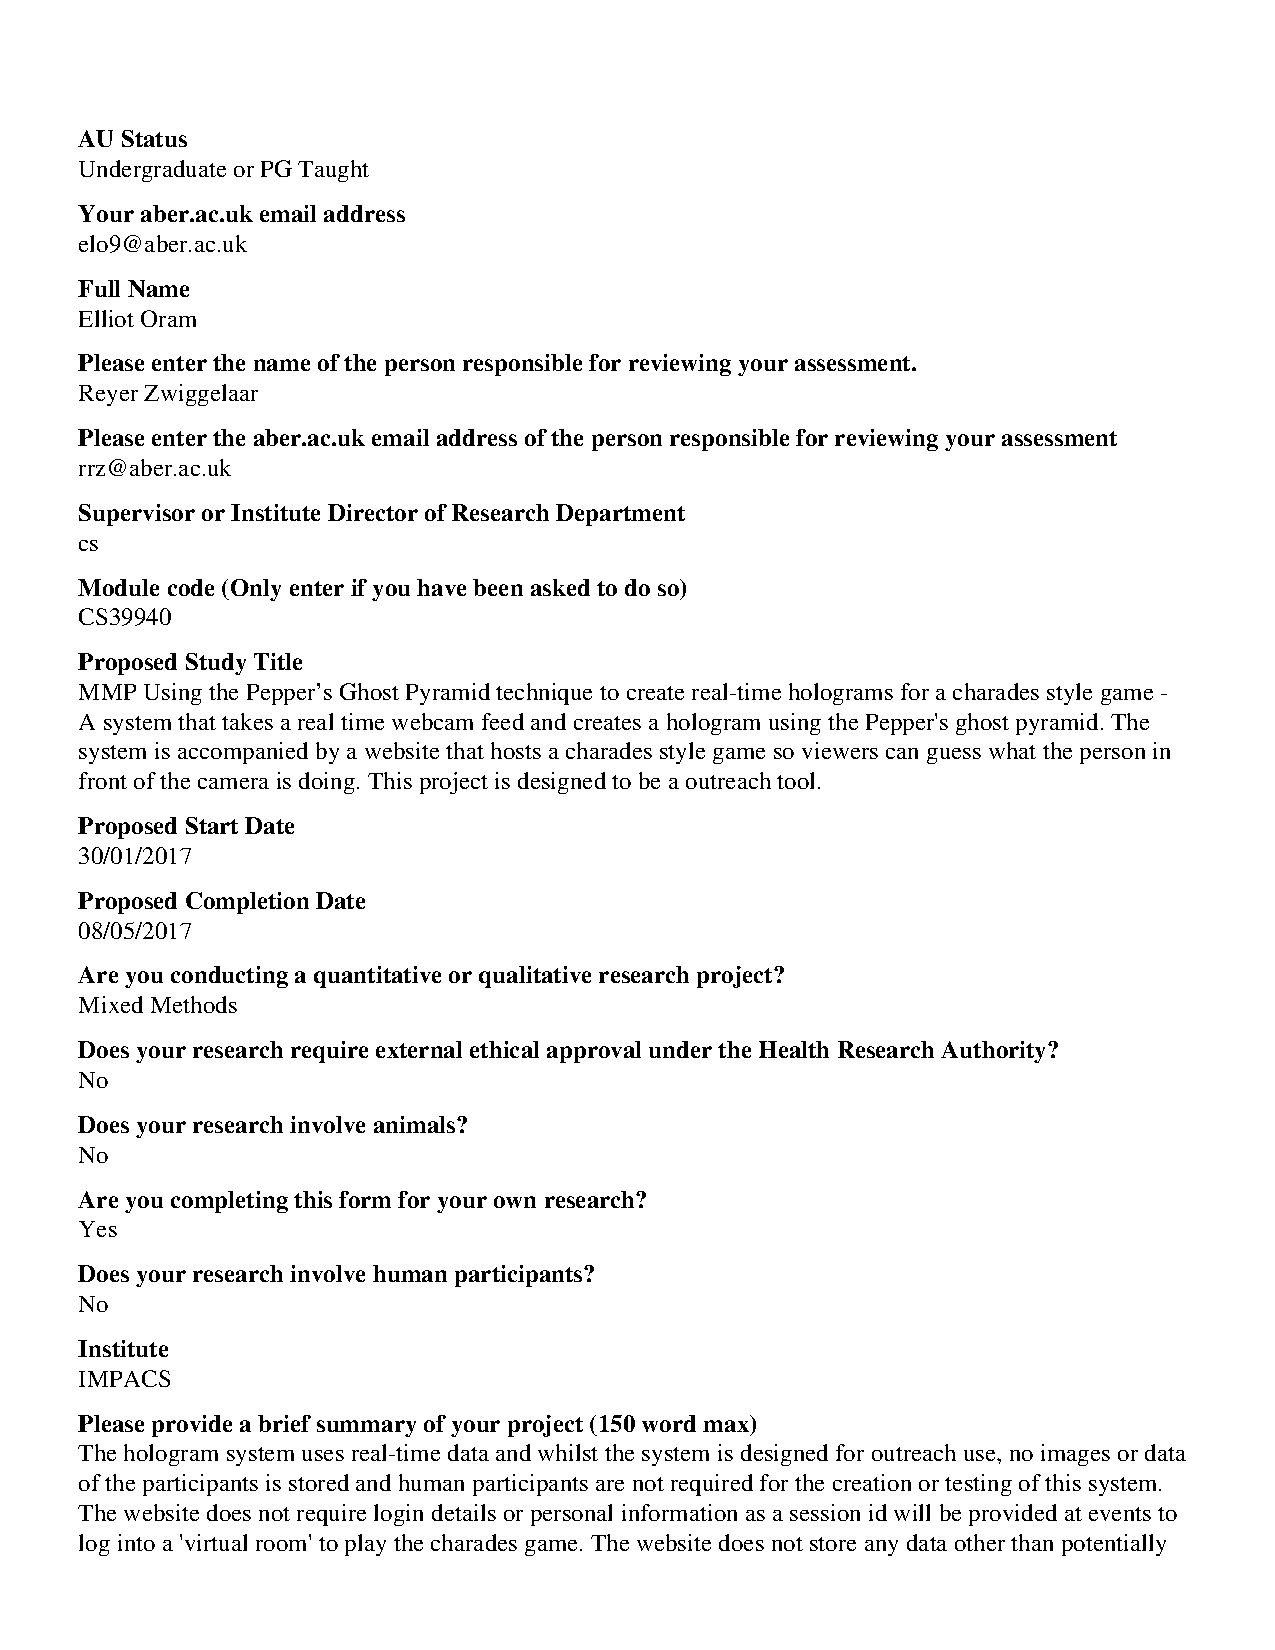
\includepdf[pages={1,2}]{Appendix2/ethics_form.pdf}


\chapter{Code Examples}

\section{Embedded Python}

The code shown below is embedded Python code taken from the acting.html template of the Charades Game. The code below is designed to change the colour of each word in the current phrase depending on if it has been guessed, it is the current word or it has yet to be used.

\begin{itemize}
	\item The use of '{\% \%}' denote a Python block where the code inside is to be executed upon page load. 
	
	\item 'forloop.counter' and 'forloop.counter0' are internal counters used to index the current position in the for loop. 'forloop.counter0' is a counter starting from 0 and 'forloop.counter' is a counter starting from 1.

\end{itemize}

\begin{verbatim}
<h1 class="page_title">


<span class="current_word_span">

<span class="completed_word_span">

<span class="word_span">

{{word}}</span>

</h1>
\end{verbatim}

\section{phrase\_ready API}

The Charades Game API function that displays if the phrase is currently in a guessable state within the system. The function is from the charades\/charades\/views.py and is discussed in Chapter 3: Iteration 7.

\begin{verbatim}
def phrase_ready_api(request):
    """
    Asserts if the phrase is ready. Only intended for api access
    """
    phrase_ready = False
    if GAME is not None:
        if GAME.actor is not None:
            phrase_ready = GAME.actor.phrase_ready()
    return render(request,
    		      'phrase_ready.html',
    		      {'phrase_ready' : phrase_ready})
\end{verbatim}


\newpage


\section{Polling function}

The JavaScript and JQuery function used to retrieve data from the guess\_correct API. The function is from the file charades\/templates\/guess.html and discussed in Chapter 3: Iteration 7.

\begin{verbatim}
<script
src="https://ajax.googleapis.com/ajax/libs/jquery/3.2.0/jquery.min.js">
</script>
<script>
setInterval(function(){
    $.get( "/api/guess_correct", function( data ) {
        if (data.includes("Word") || data.includes("Phrase")) {
            window.location.replace('/waiting_for_actor/');
        }
    });
    poll();
}, 1000);
</script>
\end{verbatim}
\chapter{UI diagrams}

\section{Index}
\begin{figure}[h!]
	\centering{
		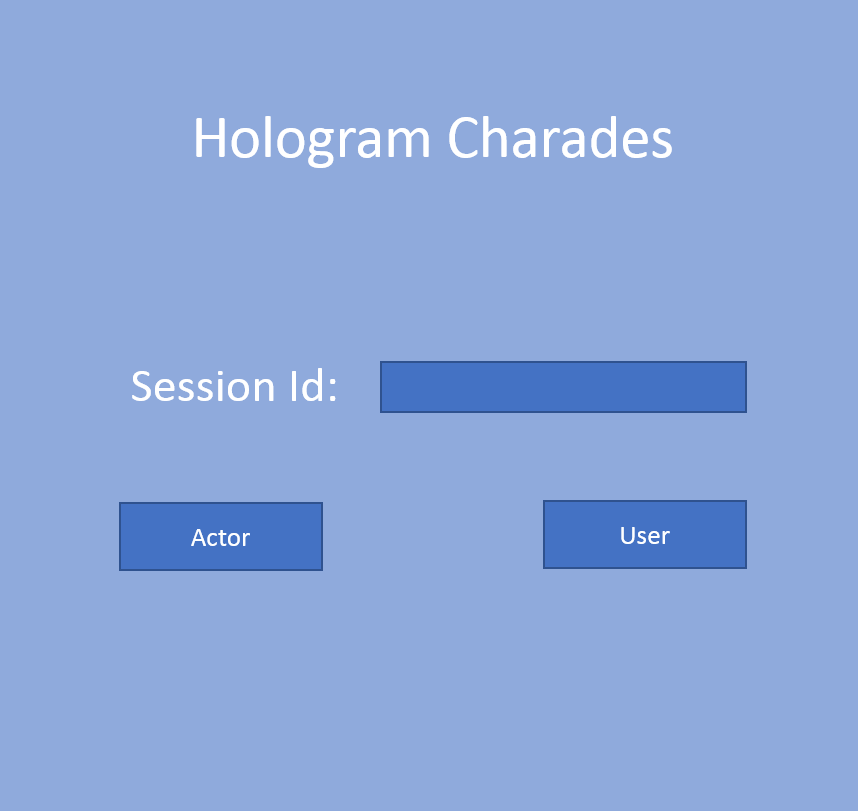
\includegraphics[scale=0.6]{Appendix4/index.png}
	}
\end{figure}

The landing page for the Charades Game.

\newpage

\section{Instructions}
\begin{figure}[h!]
	\centering{
		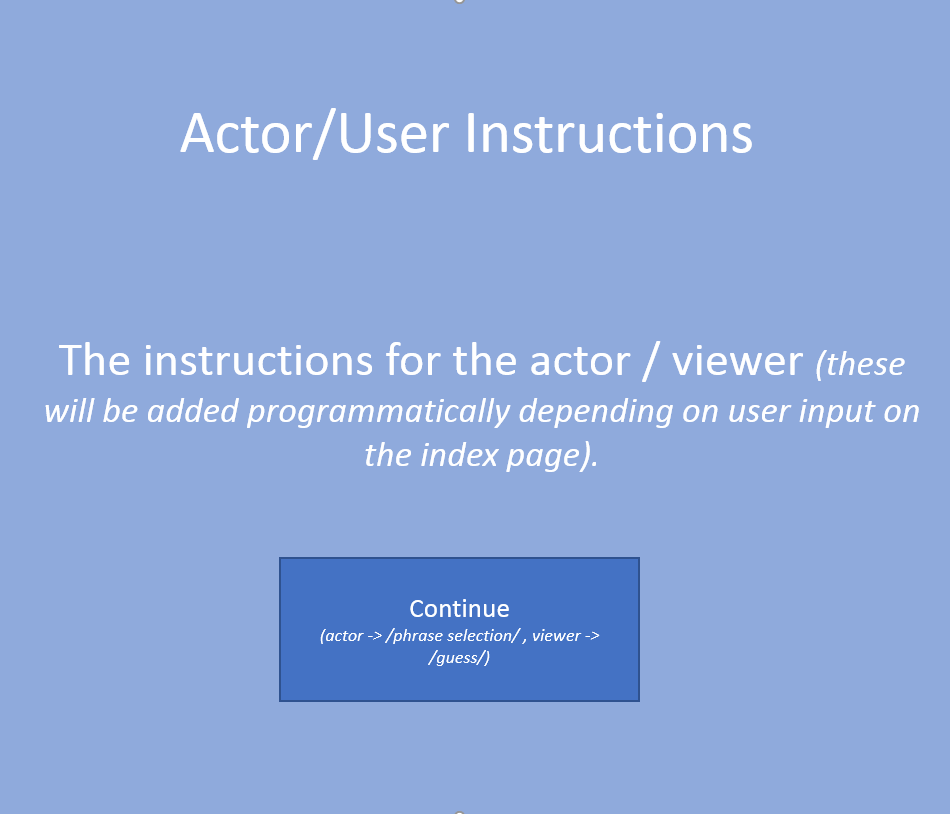
\includegraphics[scale=0.6]{Appendix4/instructions.png}
	}
\end{figure}
The instruction screen for the actor and viewer.

\newpage

\section{Select\_phrase}
\begin{figure}[h!]
	\centering{
		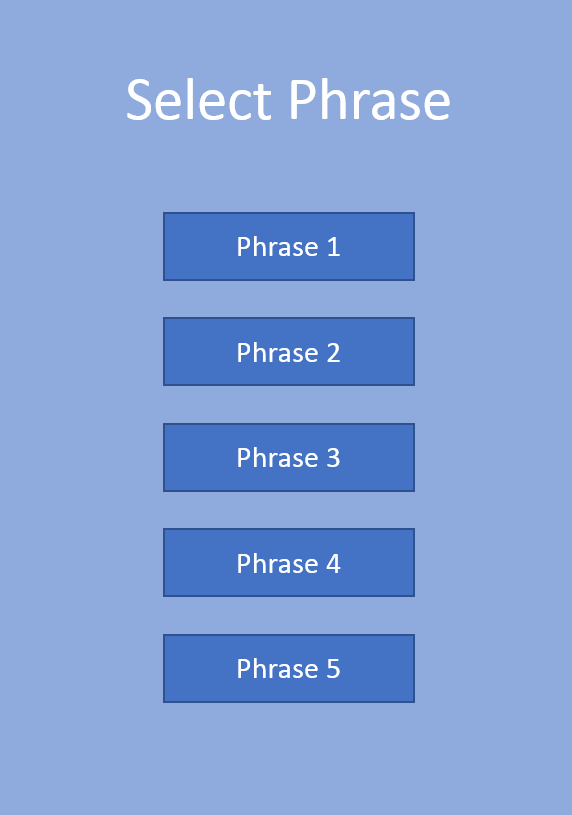
\includegraphics[scale=0.6]{Appendix4/select_phrase.png}
	}
\end{figure}
The selection screen for the actor to chose a phrase to act.

\newpage

\section{Acting\_single\_word}
\begin{figure}[h!]
	\centering{
		
\includegraphics[scale=0.6]{Appendix4/acting_single_word.png}
	}
\end{figure}
The acting screen for when there is only one word in the phrase.

\newpage

\section{Acting\_multi\_word}
\begin{figure}[h!]
	\centering{
		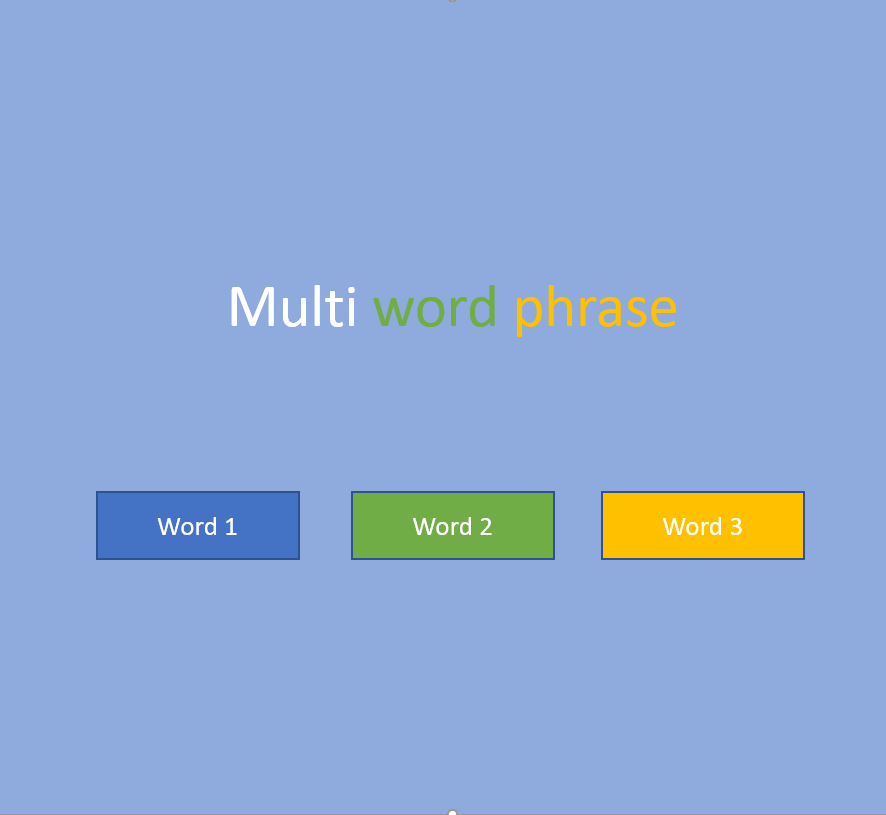
\includegraphics[scale=0.6]{Appendix4/acting_mulit_word.png}
	}
\end{figure}
The actors word selection screen when the phrase is comprised of multiple words. Green is if the word is complete. Yellow if for the currently selected word. Blue/white is unselected words.

\newpage


\section{Waiting\_for\_actor}
\begin{figure}[h!]
	\centering{
		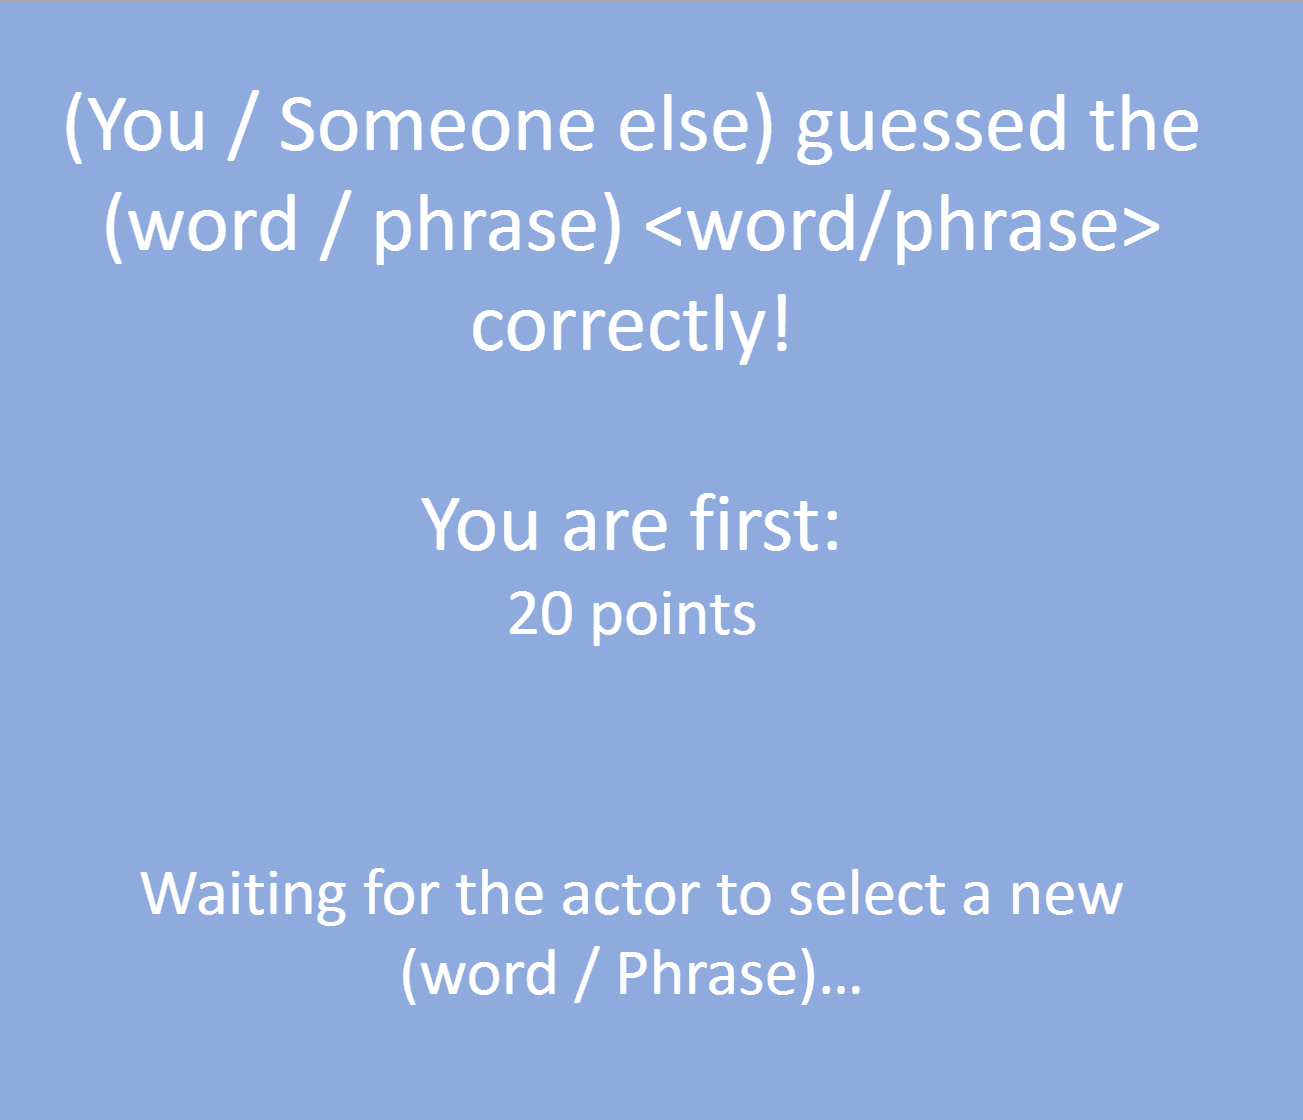
\includegraphics[scale=0.4]{Appendix4/waiting_for_actor.png}
	}
\end{figure}
The page that is displayed while the viewer waits for the actor to select an new word or phrase.

\newpage

\fancypagestyle{plain}{%
   \fancyhead{} %[C]{Annotated Bibliography}
   \fancyfoot[C]{{\thepage} of \pageref{LastPage}} % except the center
   \renewcommand{\headrulewidth}{0pt}
   \renewcommand{\footrulewidth}{0pt}
}

\setemptyheader

\nocite{*} % include everything from the bibliography, irrespective of whether it has been referenced.

% the following line is included so that the bibliography is also shown in the table of contents. There is the possibility that this is added to the previous page for the bibliography. To address this, a newline is added so that it appears on the first page for the bibliography. 
\addcontentsline{toc}{chapter}{Annotated Bibliography} % Adds References to contents page

%
% example of including an annotated bibliography. The current style is an author date one. If you want to change, comment out the line and uncomment the subsequent line. You should also modify the packages included at the top (see the notes earlier in the file) and then trash your aux files and re-run. 
%\bibliographystyle{authordate2annot}
\bibliographystyle{IEEEannotU}
\renewcommand{\bibname}{Annotated Bibliography} 

\bibliography{References/references} % References file

\end{document}
